%Este trabalho está licenciado sob a Licença Atribuição-CompartilhaIgual 4.0 Internacional Creative Commons. Para visualizar uma cópia desta licença, visite http://creativecommons.org/licenses/by-sa/4.0/deed.pt_BR ou mande uma carta para Creative Commons, PO Box 1866, Mountain View, CA 94042, USA.

\chapter{Produto vetorial}\label{cap_prodvet}
\badgeRevisar

De agora em diante, vamos trabalhar com um base ortonormal $B = (\vec{i}, \vec{j}, \vec{k})$ dita com orientação positiva, i.e. os vetores $\vec{i} = \overrightarrow{OI}$, $\vec{j} = \overrightarrow{OJ}$ e $\vec{k}=\overrightarrow{OK}$ estão dispostos em sentido anti-horário, veja Figura \ref{fig:base_pos}.

\begin{figure}[H]
  \centering
  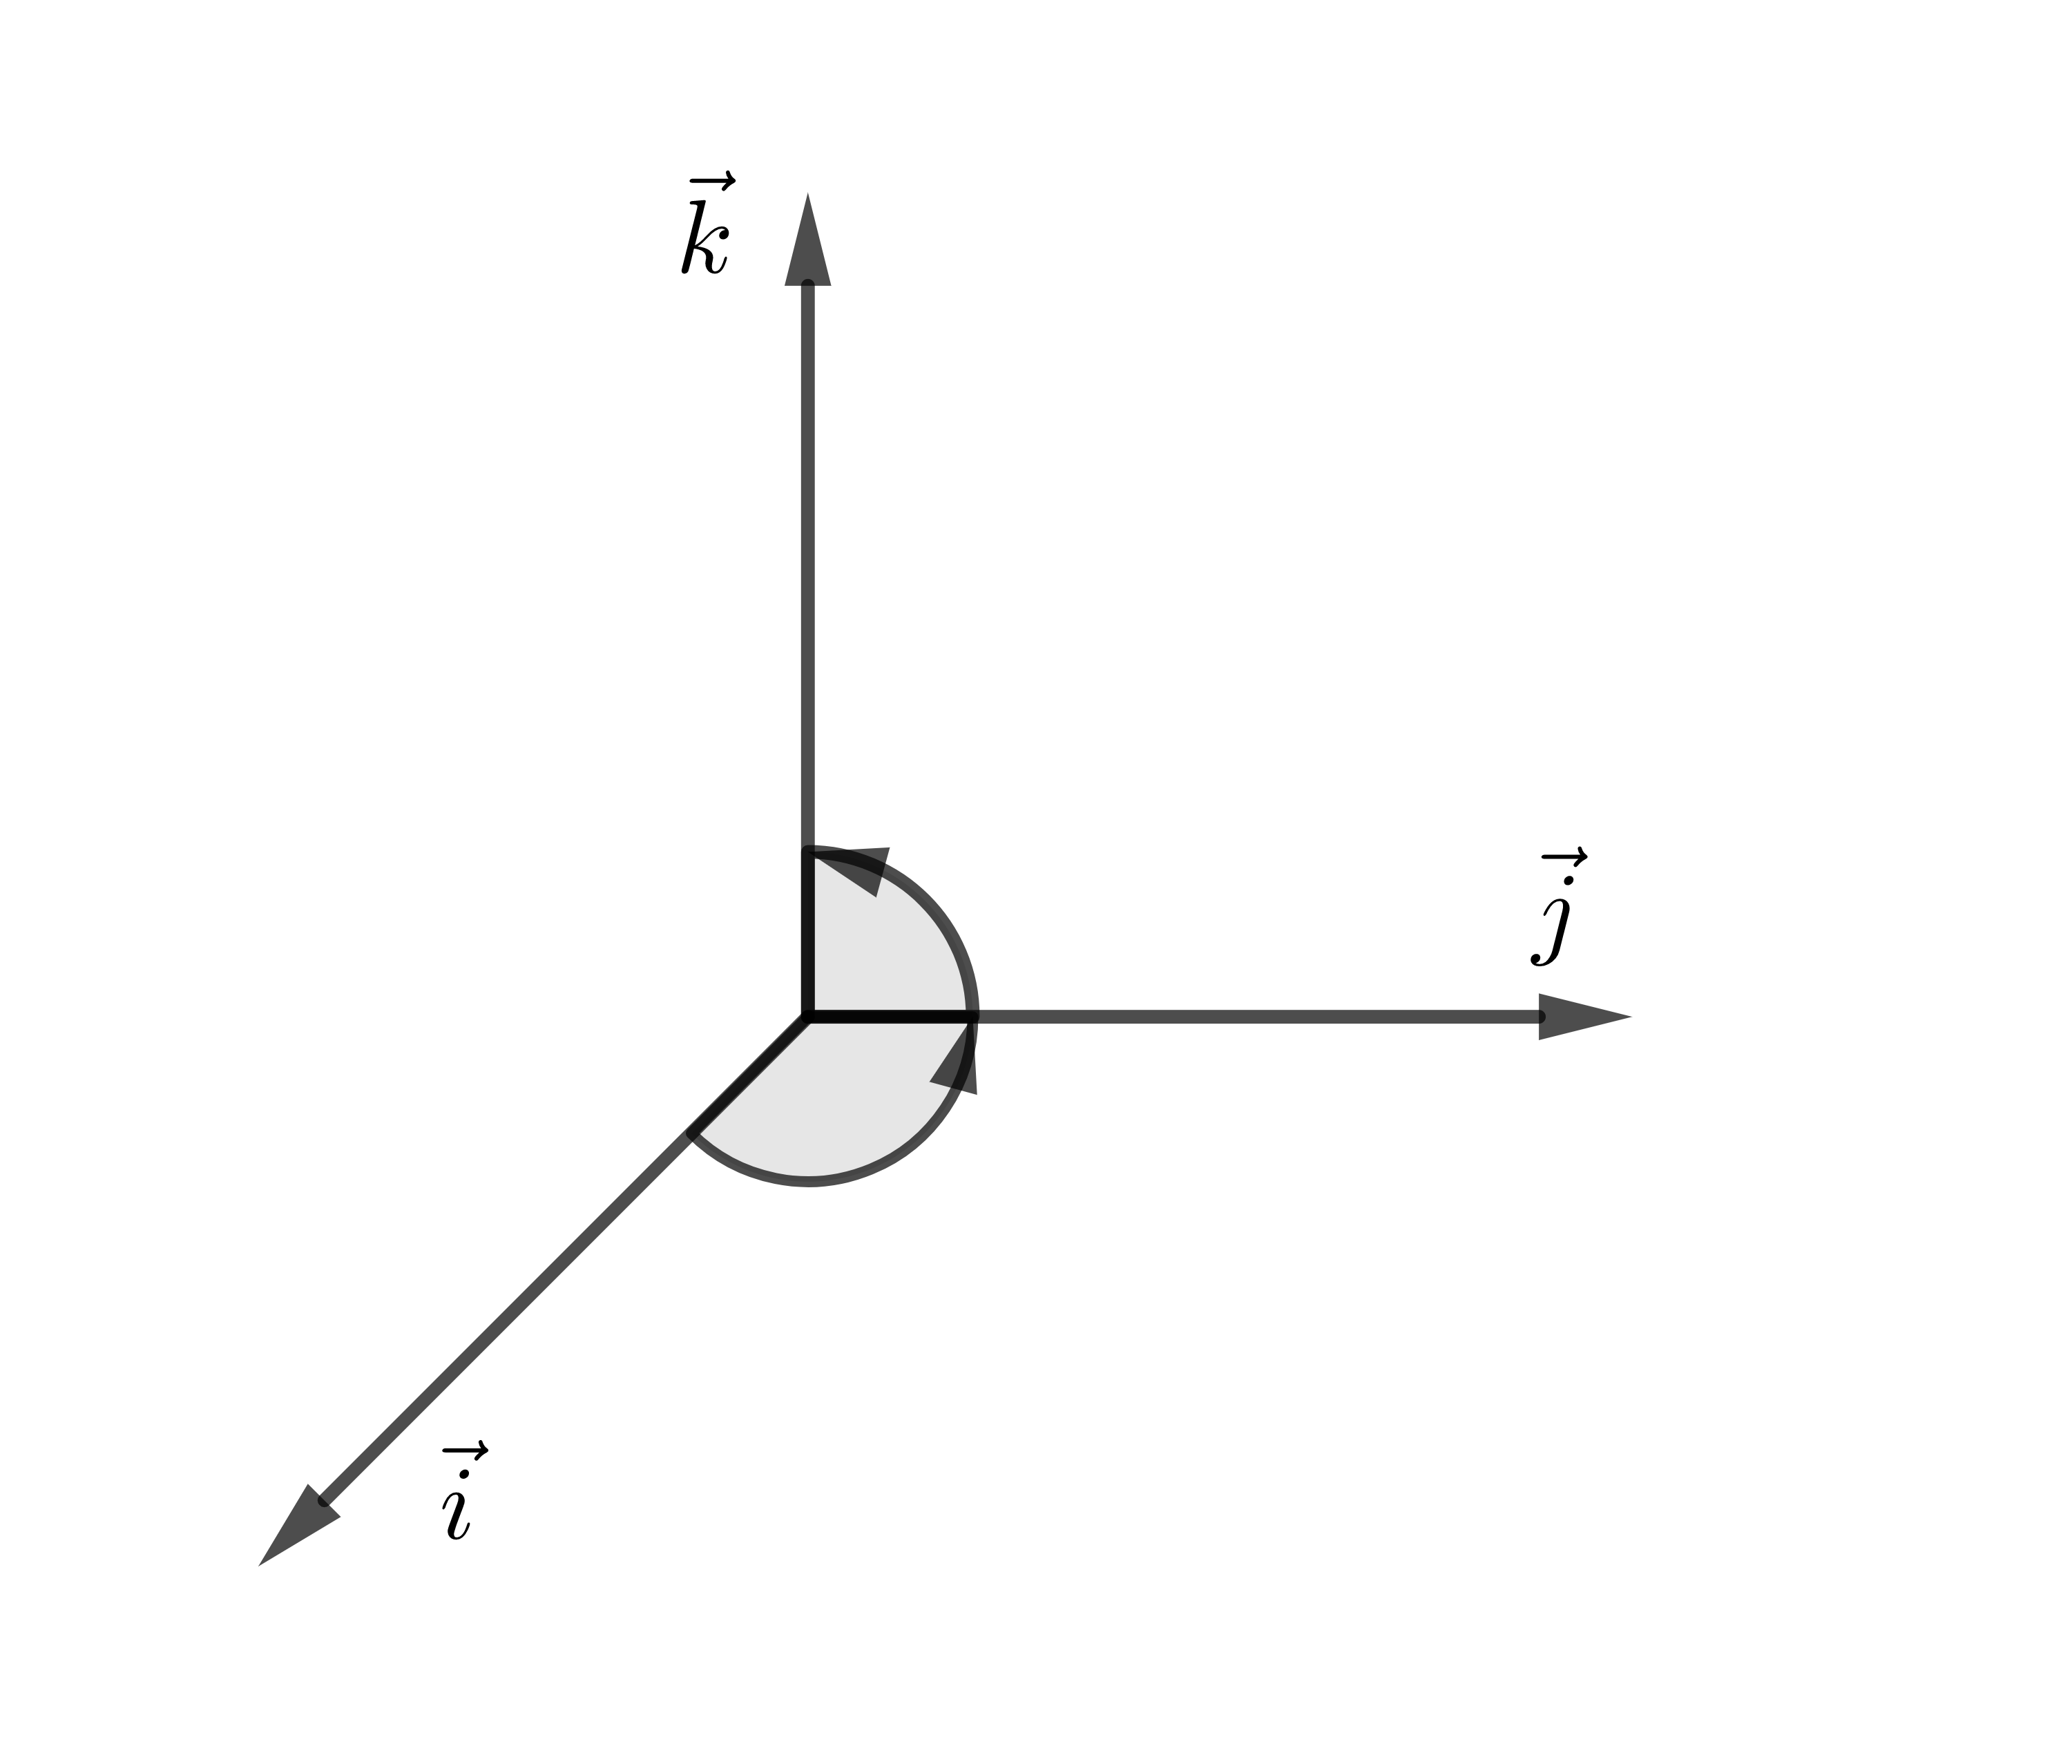
\includegraphics[width=0.7\textwidth]{./cap_prodvet/dados/fig_base_pos/fig_base_pos}
  \caption{Base ortonormal positiva.}
  \label{fig:base_pos}
\end{figure}

\section{Definição}\label{cap_prodvet_sec_prodvet}
\badgeRevisar

Dados vetores $\vec{u}$ e $\vec{v}$, definimos o produto vetorial de $\vec{u}$ com $\vec{v}$, denotado por $\vec{u}\land\vec{v}$, como o vetor:
\begin{itemize}
\item se $\vec{u}$ e $\vec{v}$ são l.d., então $\vec{u}\land\vec{v} = \vec{0}$.
\item se $\vec{u}$ e $\vec{v}$ são l.i., então
  \begin{itemize}
  \item $|\vec{u}\land\vec{v}| = |\vec{u}||\vec{v}|\sen\alpha$, onde $\alpha$ é o ângulo entre $\vec{u}$ e $\vec{v}$,
  \item $\vec{u}\land\vec{v}$ é ortogonal a $\vec{u}$ e $\vec{v}$, e
  \item $\vec{u}$, $\vec{v}$ e $\vec{u}\land\vec{v}$ formam uma base positiva.
  \end{itemize}
\end{itemize}

\subsection{Interpretação geométrica}

Sejam dados $\vec{u}$ e $\vec{v}$ l.i.. Estes vetores determinam um paralelogramo, veja Figura \ref{fig:prodvet_interp} (esquerda). Seja, então, $h$ a altura deste paralelogramo tendo $\vec{u}$ como sua base. Logo, a área do paralelogramo é o produto do comprimento da base com sua altura, neste caso
\begin{align}
  |\vec{u}|h &= |\vec{u}||\vec{v}|\sen\alpha\\
             &= |\vec{u}\land\vec{v}|
\end{align}
Ou seja, o produto vetorial $\vec{u}\land\vec{v}$ tem norma igual à área do paralelogramo determinado por $\vec{u}$ e $\vec{v}$.

Ainda, por definição, $\vec{u}\land\vec{v}$ é ortogonal a $\vec{u}$ e $\vec{v}$. Isto nos dá a direção de $\vec{u}\land\vec{v}$. O sentido é, então, determinado pela definição de que $(\vec{u},\vec{v},\vec{u}\land\vec{v})$ é uma base positiva. Veja a Figura \ref{fig:prodvet_interp} (direita).

\begin{figure}[H]
  \centering
  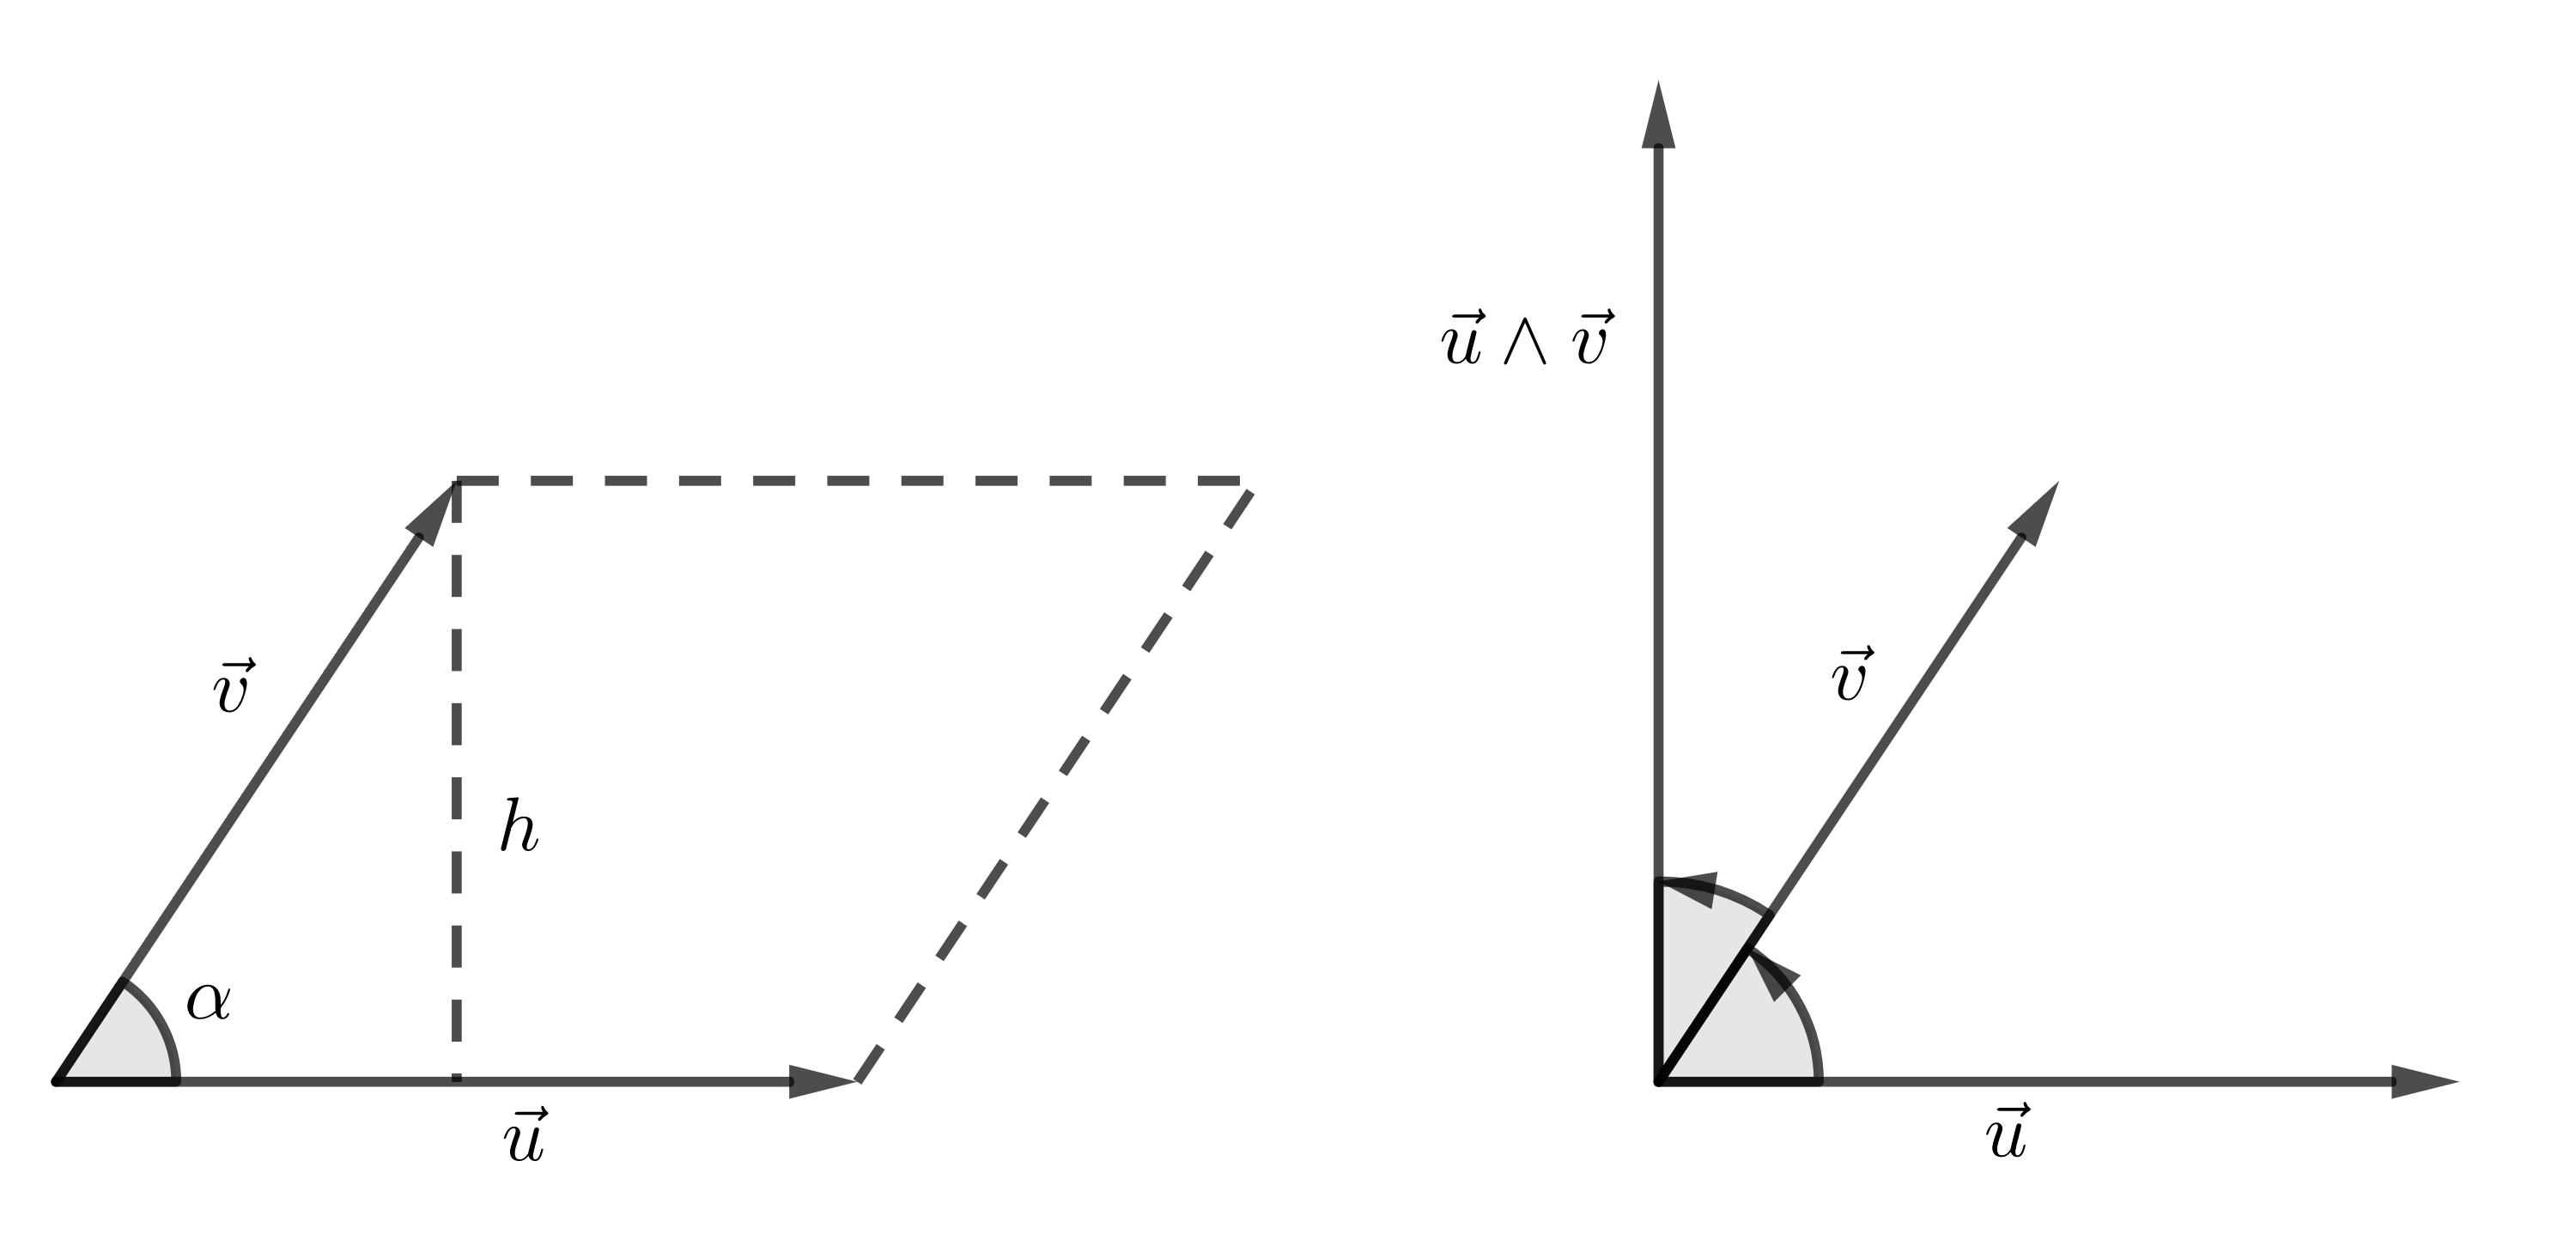
\includegraphics[width=0.7\textwidth]{./cap_prodvet/dados/fig_prodvet_interp/fig_prodvet_interp}
  \caption{Interpretação do produto vetorial.}
  \label{fig:prodvet_interp}
\end{figure}

\subsection{Produto vetorial via coordenadas}\label{cap_prodvet_sec_coord}

Dados $\vec{u} = (u_1,u_2,u_3)$ e $\vec{v} = (v_1,v_2,v_3)$ em uma base ortonormal positiva, então
\begin{equation}
  \vec{u}\land\vec{v} =
  \begin{vmatrix}
    u_2 & u_3\\
    v_2 & v_3
  \end{vmatrix}\vec{i} -
  \begin{vmatrix}
    u_1 & u_3\\
    v_1 & v_3
  \end{vmatrix}\vec{j} +
  \begin{vmatrix}
    u_1 & u_2 \\
    v_1 & v_2
  \end{vmatrix}\vec{k}.
\end{equation}

\begin{obs}
  Uma regra mnemônica, é
  \begin{equation}
    \vec{u}\land\vec{v} =
    \begin{vmatrix}
      \vec{i} & \vec{j} & \vec{k} \\
      u_1 & u_2 & u_3 \\
      v_1 & v_2 & v_3
    \end{vmatrix}.
  \end{equation}
\end{obs}

\begin{ex}
  Dados os vetores $\vec{u} = (1,-2,1)$ e $\vec{v} = (0,2,-1)$, temos
  \begin{align}
    \vec{u}\land\vec{v} &=
                          \begin{vmatrix}
                            \vec{i} & \vec{j} & \vec{k} \\
                            u_1 & u_2 & u_3 \\
                            v_1 & v_2 & v_3
                          \end{vmatrix} \\
                        &=
                          \begin{vmatrix}
                            \vec{i} & \vec{j} & \vec{k} \\
                            1       & -2      & 1 \\
                            0       & 2       & -1
                          \end{vmatrix} \\
                        &= 0\vec{i} + \vec{j} + 2\vec{k}\\
                        &= (0,1,2).
  \end{align}
\end{ex}

\subsection*{Exercícios resolvidos}

\begin{exeresol}
  Calcule $\vec{x}$ tal que $(0,2,-1)\land\vec{x}=(-3,-1,-2)$.
\end{exeresol}
\begin{resol}
  Denotando $\vec{x}=(x_1,x_2,x_3)$, temos
  \begin{gather}
    (0,2,-1)\land\vec{x}=(-3,-1,-2)\\
    \begin{vmatrix}
      \vec{i} & \vec{j} & \vec{k} \\
      0 & 2 & -1 \\
      x_1 & x_2 & x_3
    \end{vmatrix} = (-3,-1,-2)\\
    (x_2+2x_3)\vec{i}-x_1\vec{j}-2x_1\vec{k} = \\
    -3\vec{i}-\vec{j}-2\vec{k}
  \end{gather}
  Segue que
  \begin{align*}
    x_2+2x_3 &= -3\\
    -x_1 &= -1\\
    -2x_1 &= -2
  \end{align*}
  Logo, $x_1 = 1$, $x_2=-3-2x_3$ e $x_3$ é arbitrário. Concluímos que $\vec{x} = (1,-3-2x_3,x_3)$ com $x_3\in\mathbb{R}$.
\end{resol}

\begin{exeresol}
  Determine a área do paralelogramo determinado pelos vetores $\vec{u} = (-1, 2, 3)$ e $\vec{v} = (1,-2,1)$.
\end{exeresol}
\begin{resol}
  Tomando representações $\vec{u}=\overrightarrow{OA}$ e $\vec{v}=\overrightarrow{OC}$, temos que $\vec{u}$ e $\vec{v}$ determinam um paralelogramo $OABC$, onde $C$ é tal que $\vec{u}+\vec{v}=\overrightarrow{OB}$\footnote{Veja a regra do paralelogramo na Observação \ref{obs:vetor_regra_do_paralelogramo}.}. Da definição do produto vetorial, temos que
  \begin{equation}
    |\vec{u}\land\vec{v}| = |\vec{u}||\vec{v}|\sen\alpha,
  \end{equation}
  o que é igual a área do paralelogramo $OABC$, onde $\alpha$ é o ângulo entre os vetores $\vec{u}$ e $\vec{v}$. Logo, a área do paralelogramo é
  \begin{gather}
    |\vec{u}\land\vec{v}| =
    \begin{vmatrix}
      \vec{i} & \vec{j} & \vec{k} \\
      -1 & 2 & 3 \\
      1 & -2 & 1
    \end{vmatrix}\\
    |\vec{u}\land\vec{v}| = |(8,4,0)|\\
    |\vec{u}\land\vec{v}| = 4\sqrt{5}
  \end{gather}
\end{resol}

\subsection*{Exercícios}

\begin{exer}
  Sejam $\vec{u}=(2,-3,1)$ e $\vec{v}=(1,-2,-1)$. Calcule:
  \begin{enumerate}[a)]
  \item $\vec{u}\land\vec{v}$.
  \item $\vec{v}\land\vec{u}$.
  \item $\vec{v}\land(2\vec{u})$.
  \end{enumerate}
\end{exer}
\begin{resp}
  a)~$(5,3,-1)$; b)~$(-5,-3,1)$; c)~$(-10,-6,2)$
\end{resp}

\begin{exer}
  Sejam $\vec{u}$ e $\vec{v}$ tais que $\vec{u}\land\vec{v}=(2,-1,0)$. Forneça $\vec{v}\land\vec{u}$. Justifique sua resposta.
\end{exer}
\begin{resp}
  $(-2,1,0)$
\end{resp}

\begin{exer}
  Seja $\vec{u}$ um vetor qualquer. Calcule $\vec{u}\land\vec{u}$.
\end{exer}
\begin{resp}
  $0$
\end{resp}

\begin{exer}
  Sejam $\vec{u}$ e $\vec{v}$ tais que $(2\vec{u})\land\vec{v}=(2,-1,0)$. Forneça $\vec{v}\land\vec{u}$. Justifique sua resposta.
\end{exer}
\begin{resp}
  $(-1,1/2,0)$
\end{resp}

\begin{exer}
  Calcule $\vec{x}$ tal que $\vec{x}\land (2,-2,3)=(11,8,2)$.
\end{exer}
\begin{resp}
  $\left(-\frac{2}{3}x_3+\frac{8}{3},\frac{2}{3}x_3-\frac{11}{3},x_3\right), x_3\in\mathbb{R}$
\end{resp}

\begin{exer}
  Seja $B=(\vec{i},\vec{j},\vec{k})$ uma base ortonormal positiva. Calcule:
  \begin{enumerate}[a)]
  \item $\vec{i}\land\vec{j}$
  \item $\vec{j}\land\vec{k}$
  \item $\vec{k}\land\vec{i}$
  \end{enumerate}
\end{exer}
\begin{resp}
  a)~$\vec{k}$; b)~$\vec{i}$; c)~$\vec{j}$
\end{resp}

\section{Propriedades do produto vetorial}\label{cap_prodvet_sec_prop}
\badgeRevisar

Nesta seção, discutiremos sobre algumas propriedades do produto vetorial. Para tanto, sejam dados os vetores $\vec{u} = (u_1,u_2,u_3)$, $\vec{v}=(v_1,v_2,v_3)$, $\vec{w}=(w_1,w_2,w_3)$ e o número real $\gamma$.

Da definição do produto vetorial, temos $\vec{u}\perp(\vec{u}\land\vec{v})$ e $\vec{v}\perp(\vec{u}\land\vec{v})$, logo
\begin{equation}
  {\color{blue}\vec{u}\cdot(\vec{u}\land\vec{v}) = 0}
\end{equation}
e
\begin{equation}
  {\color{blue}\vec{v}\cdot(\vec{u}\land\vec{v}) = 0}.
\end{equation}

\begin{ex}
  Sejam $\vec{u}=(1,-1,2)$, $\vec{v}=(2,-1,-2)$. Temos
  \begin{align}
    \vec{u}\land\vec{v} &=
    \begin{vmatrix}
      \vec{i} & \vec{j} & \vec{k} \\
      1 & -1 & 2 \\
      2 & -1 & -2
    \end{vmatrix}\\
              &= (4,6,1)
  \end{align}
  Segue, que
  \begin{align}
    \vec{u}\cdot(\vec{u}\land\vec{v}) &= (1,-1,2)\cdot (4,6,1) \\
                                      &= 4-6+2\\
                                      &= 0.
  \end{align}
\end{ex}

Em relação à multiplicação por escalar, temos
\begin{align}
  {\color{blue}\gamma(\vec{u}\land\vec{v})} &= {\color{red}(\gamma\vec{u})\land\vec{v}} \\
                              &= {\color{cyan}\vec{u}\land(\gamma\vec{v})}.
\end{align}
De fato,
\begin{align}
  {\color{red}(\gamma\vec{u})\land\vec{v}} &=
                                {\color{red}\begin{vmatrix}
                                  \vec{i} & \vec{j} & \vec{k} \\
                                  \gamma u_1 & \gamma u_2 & \gamma u_3\\
                                  v_1 & v_2 & v_3
                                \end{vmatrix}} \\
                              &= {\color{blue}\gamma\begin{vmatrix}
                                  \vec{i} & \vec{j} & \vec{k} \\
                                  u_1 & u_2 & u_3\\
                                  v_1 & v_2 & v_3
                                \end{vmatrix}} = {\color{blue}\gamma(\vec{u}\land\vec{v})}\\
                              &=
                                {\color{cyan}\begin{vmatrix}
                                  \vec{i} & \vec{j} & \vec{k} \\
                                  u_1 & u_2 & u_3\\
                                  \gamma v_1 & \gamma v_2 & \gamma v_3
                                \end{vmatrix}} = {\color{cyan}\vec{u}\land(\gamma\vec{v})}
\end{align}

\begin{ex}
  Sejam $\vec{u}=(1,-1,2)$ e $\vec{v}=(2,-1,-2)$. Temos
  \begin{align}
    {\color{blue}2(\vec{u}\land\vec{v})} &=
    2\begin{vmatrix}
      \vec{i} & \vec{j} & \vec{k} \\
      1 & -1 & 2 \\
      2 & -1 & -2
    \end{vmatrix}\\
                           &= 2(4,6,1)\\
                           &= (8,12,2)
  \end{align}
  \begin{align}
    {\color{red}(2\vec{u})\land\vec{v}} &=
    \begin{vmatrix}
      \vec{i} & \vec{j} & \vec{k} \\
      2 & -2 & 4 \\
      2 & -1 & -2
    \end{vmatrix}\\
                           &= (8,12,2)
  \end{align}
  \begin{align}
    {\color{cyan}\vec{u}\land(2\vec{v})} &=
    \begin{vmatrix}
      \vec{i} & \vec{j} & \vec{k} \\
      1 & -1 & 2 \\
      4 & -2 & -4
    \end{vmatrix}\\
                           &= (8,12,2)
  \end{align}
\end{ex}


Também, vale a {\color{blue}propriedade distributiva com a operação de soma}, i.e.
\begin{equation}
  {\color{blue}\vec{u}\land(\vec{v} + \vec{w}) = \vec{u}\land\vec{v}+\vec{u}\land\vec{w}}.
\end{equation}
De fato, temos
\begin{gather}
  \vec{u}\land(\vec{v}+\vec{w}) \\
  = \begin{vmatrix}
    \vec{i} & \vec{j} & \vec{k} \\
    u_1 & u_2 & u_3 \\
    v_1+w_1 & v_2+w_2 & u_3+w_3
  \end{vmatrix} \\
  = \begin{vmatrix}
    \vec{i} & \vec{j} & \vec{k} \\
    u_1 & u_2 & u_3 \\
    v_1 & v_2 & v_3
  \end{vmatrix}
  +  \begin{vmatrix}
    \vec{i} & \vec{j} & \vec{k} \\
    u_1 & u_2 & u_3 \\
    w_1 & w_2 & w_3
  \end{vmatrix}\\
  = \vec{u}\land\vec{v} + \vec{u}\land\vec{w}.
\end{gather}

\begin{ex}
  Sejam $\vec{u}=(1,-1,2)$, $\vec{v}=(2,-1,-2)$ e $\vec{w}=(0,-1,-1)$. Temos
  \begin{gather}
    \vec{u}\land(\vec{v}+\vec{w}) \\
    = \vec{u}\land \left[(2,-1,-2)+(0,-1,-1)\right]
    = (1,-1,2)\land (2,-2,-3) \\
    = \begin{vmatrix}
      \vec{i} & \vec{j} & \vec{k} \\
      1 & -1 & 2 \\
      2 & -2 & -3
    \end{vmatrix} \\
    = (7,7,0)  
  \end{gather}
  \begin{gather}
    (\vec{u}\land\vec{v}) + (\vec{u}\land\vec{w}) \\
        = \begin{vmatrix}
          \vec{i} & \vec{j} & \vec{k} \\
          1 & -1 & 2 \\
          2 & -1 & -2
        \end{vmatrix} + \begin{vmatrix}
          \vec{i} & \vec{j} & \vec{k} \\
          1 & -1 & 2 \\
          0 & -1 & -1
        \end{vmatrix} \\
        = (4,6,1) + (3,1,-1) \\
        = (7,7,0)
  \end{gather}
\end{ex}

Observamos que o {\color{blue}produto vetorial não é comutativo}, entretanto
\begin{equation}
  {\color{blue}\vec{u}\land\vec{v} = -\vec{v}\land\vec{u}}.
\end{equation}
De fato, temos
\begin{gather}
  \vec{u}\land\vec{v} \\
  = \begin{vmatrix}
    \vec{i} & \vec{j} & \vec{k} \\
    u_1 & u_2 & u_3 \\
    v_1 & v_2 & v_3                                    
  \end{vmatrix}\\
  = -\begin{vmatrix}
    \vec{i} & \vec{j} & \vec{k} \\
    v_1 & v_2 & v_3 \\
    u_1 & u_2 & u_3                                    
  \end{vmatrix}\\
  = -\vec{v}\land\vec{u}.
\end{gather}

\begin{ex}
  Sejam $\vec{u}=(1,-1,2)$ e $\vec{v}=(2,-1,-2)$. Temos
  \begin{align}
    \vec{u}\land\vec{v} \\
    &= \begin{vmatrix}
      \vec{i} & \vec{j} & \vec{k} \\
      1 & -1 & 2 \\
      2 & -1 & -2                                    
    \end{vmatrix} \\
    &= (4,6,1)
  \end{align}
  \begin{align}
    \vec{v}\land\vec{u} \\
    &= \begin{vmatrix}
      \vec{i} & \vec{j} & \vec{k} \\
      2 & -1 & -2 \\
      1 & -1 & 2
    \end{vmatrix} \\
    &= (-4,-6,-1)
  \end{align}
\end{ex}

Também, o {\color{blue}produto vetorial não é associativo} sendo $(\vec{u}\land\vec{v})\land\vec{w}$, em geral, é diferente de $\vec{u}\land(\vec{v}\land\vec{w})$. Com efeito, temos
\begin{align}
  {\color{blue}(\vec{i}\land\vec{i})\land\vec{j}} &= \vec{0},\\
  {\color{blue}\vec{i}\land(\vec{i}\land\vec{j})} &= \vec{i}\land\vec{k} = -\vec{j}.
\end{align}

Por outro lado, suponhamos que $\vec{u}$, $\vec{v}$ e $\vec{w}$ são l.i. e seja $\pi$ um plano determinado por $\vec{u}$ e $\vec{v}$. Então, $\vec{u}\land\vec{v}$ é ortogonal a $\pi$. Como $(\vec{u}\land\vec{v})\land\vec{w}$ é ortogonal a $\vec{u}\land\vec{v}$ e a $\vec{w}$, temos que $(\vec{u}\land\vec{v})\land\vec{w}$ também pertence a $\pi$. Logo, $\vec{u}$, $\vec{v}$ e $(\vec{u}\land\vec{v})\land\vec{w}$ são l.d. e existem $\alpha$ e $\beta$ tais que
\begin{equation}
  {\color{blue}(\vec{u}\land\vec{v})\land\vec{w} = \alpha\vec{u} + \beta\vec{v}}.
\end{equation}
Vamos determinar $\alpha$ e $\beta$. Para tanto, consideremos uma base ortonormal $B = (\vec{i}, \vec{j}, \vec{k})$ tal que $\vec{i}\parallel\vec{u}$ e $\vec{j}\in\pi$. Nesta base, temos
\begin{align}
  \vec{u} &= (u_1,0,0)\\
  \vec{v} &= (v_1,v_2,0)\\
  \vec{w} &= (w_1,w_2,w_3).
\end{align}
Também, temos
\begin{align}
  \vec{u}\land\vec{v} &=
  \begin{vmatrix}
    \vec{i} & \vec{j} & \vec{k} \\
    u_1 & 0 & 0 \\
    v_1 & v_2 & 0
  \end{vmatrix} \\
  &= (0,0,u_1v_2)
\end{align}
e
\begin{align}
  (\vec{u}\land\vec{v})\land\vec{w} &=
                                      \begin{vmatrix}
                                        \vec{i} & \vec{j} & \vec{k} \\
                                        0 & 0 & u_1v_2 \\
                                        w_1 & w_2 & w_3
                                      \end{vmatrix}\\
                                    &= (-u_1v_2w_2,u_1v_2w_1,0).
\end{align}
Daí, temos
\begin{equation}
  \underbrace{(-u_1v_2w_2,u_1v_2w_1,0)}_{(\vec{u}\land\vec{v})\land\vec{w}} = \underbrace{\alpha(u_1,0,0)+\beta(v_1,v_2,0)}_{\alpha\vec{u}+\beta\vec{v}},
\end{equation}
donde
\begin{align}
  \alpha u_1+\beta v_1 &= -u_1v_2w_2,\\
  \beta v_2 &= u_1w_1v_2.  
\end{align}
Resolvendo para $\alpha$ e $\beta$, obtemos
\begin{align}
  \alpha &= -v_1w_1-v_2w_2 = -\vec{v}\cdot\vec{w}\\
  \beta &= \vec{u}\vec{w}.
\end{align}
Portanto, temos
\begin{equation}
  {\color{blue}(\vec{u}\land\vec{v})\land\vec{w} = -(\vec{v}\cdot\vec{w})\vec{u}+(\vec{u}\cdot\vec{w})\vec{v}}.
\end{equation}

Usando as identidades acima, obtemos
\begin{align}\label{eq:prodvet_assoc1}
  \vec{u}\land(\vec{v}\land\vec{w}) &= -(\vec{v}\land\vec{w})\land\vec{u}\\
                                    &= (\vec{w}\cdot\vec{u})\vec{v}-(\vec{v}\cdot\vec{u})\vec{w}\\
                                    &= (\vec{u}\cdot\vec{w})\vec{v}-(\vec{u}\cdot\vec{v})\vec{w}
\end{align}
ou seja,
\begin{equation}
  {\color{blue}\vec{u}\land(\vec{v}\land\vec{w}) = (\vec{u}\cdot\vec{w})\vec{v}-(\vec{u}\cdot\vec{v})\vec{w}}.
\end{equation}

\subsection*{Exercícios resolvidos}

\begin{exeresol}
  Sejam $\vec{u}=(-3,-2,-1)$, $\vec{v}=(0,1,2)$ e $\vec{w}=(-1,0,1)$. Calcule
  \begin{equation}
    (\vec{u}\land\vec{v})\land\vec{w}.
  \end{equation}
\end{exeresol}
\begin{resol}
  Seguindo a identidade \eqref{eq:prodvet_assoc1}, segue
  \begin{gather}
    (\vec{u}\land\vec{v})\land\vec{w} \\
    = -(\vec{v}\cdot\vec{w})\vec{u} + (\vec{u}\cdot\vec{w})\vec{v}\\
    = -(0+0+2)\vec{u} + (3+0-1)\vec{v}\\
    = -2(-3,-2,-1)+2(0,1,2)\\
    = (6,4,2)+(0,2,4)\\
    = (6,6,6)
  \end{gather}
\end{resol}


\begin{exeresol}
  Sejam $\vec{u}=(2,x,1)$, $\vec{v}=(-2,3,1)$ e $\vec{w}=(-3,-1,1)$. Calcule $x$ tal que
  \begin{equation}
    \vec{v}\cdot(\vec{u}\land\vec{w})=-16.
  \end{equation}
\end{exeresol}
\begin{resol}
  Por cálculo direto, temos
  \begin{gather}
    \vec{v}\cdot(\vec{u}\land\vec{w})=-16\\
    \vec{v}\cdot
    \begin{vmatrix}
      \vec{i} & \vec{j} & \vec{k}\\
      2 & x & 1 \\
      -3 & -1 & 1
    \end{vmatrix} = -16 \\
    (-2,3,1)\cdot(x+1,-5,3x-2)=-16\\
    x-19 = -16 \\
    x = 3.
  \end{gather}
\end{resol}

\subsection*{Exercícios}

\begin{exer}
  Sejam $\vec{u}=(2,-3,1)$ e $\vec{v}=(3,-2,1)$. Calcule $\vec{u}\cdot(\vec{v}\land\vec{u})$. Se $\vec{w}$ é um vetor qualquer, forneça o valor de $\vec{u}\cdot(\vec{w}\land\vec{u})$. Justifique sua resposta.
\end{exer}
\begin{resp}
  $\vec{u}\cdot(\vec{v}\land\vec{u})=0$; $\vec{u}\cdot(\vec{w}\land\vec{u})=0$
\end{resp}

\begin{exer}
  Sabendo que $\vec{u}\land\vec{v}=(1,1,1)$, calcule $\vec{u}\land(2\vec{v})$.
\end{exer}
\begin{resp}
  $(2,2,2)$
\end{resp}

\begin{exer}
  Sabendo que $\vec{u}\land\vec{v}=(1,1,1)$ e $\vec{u}\land\vec{w}=(-1,-1,-1)$, calcule $\vec{u}\land(\vec{v} + \vec{w})$.
\end{exer}
\begin{resp}
  $(0,0,0)$
\end{resp}

\begin{exer}
  Sendo $\vec{a}=(3,-1,2)$, $\vec{b}=(2,-1,-1)$, calcule $(\vec{a}\cdot\vec{k})(\vec{i}\land\vec{b})$.
\end{exer}
\begin{resp}
  $(0,2,-2)$
\end{resp}

\begin{exer}
  Calcule $\vec{w}\land(\vec{u}\land\vec{v})$, sendo $\vec{u}=(1,-1,2)$, $\vec{v}=(0,-1,1)$ e $\vec{w}=(1,0,-1)$.
\end{exer}
\begin{resp}
  $(-1,0,-1)$
\end{resp}
